\documentclass{standalone}
\usepackage{tikz}
\usepackage{verbatim}
\begin{document}
\def\layersep{2.5cm}
    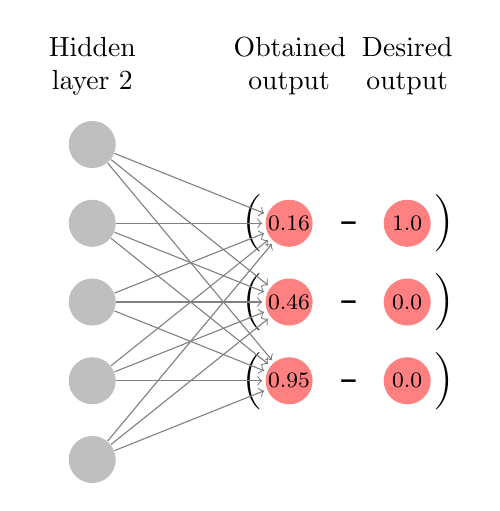
\begin{tikzpicture}[shorten >=1pt,->,draw=black!50, node distance=2.5cm]
        \tikzstyle{every pin edge}=[<-,shorten <=1pt]
        \tikzstyle{neuron}=[
            circle,fill=black!25,minimum size=17pt,inner sep=0pt, font=\footnotesize,
        ]
        \tikzstyle{output neuron}=[neuron, fill=red!50];
        \tikzstyle{hidden neuron}=[neuron, fill=gray!50];
        \tikzstyle{annot} = [text width=4em, text centered]

        % Draw the hidden layers nodes
        \foreach \id in {1,...,5}
            \path[yshift=0.5cm]
                node[hidden neuron] (H2-\id) at (1cm,-\id cm) {};

        % Draw the output layer nodes
        \node[output neuron,label={}, right of=H2-2] (Oo-1) {0.16};
        \node[output neuron,label={}, right of=H2-3] (Oo-2) {0.46};
        \node[output neuron,label={}, right of=H2-4] (Oo-3) {0.95};
        
        \node[left of=Oo-1, node distance=13] {\huge(};
        \node[left of=Oo-2, node distance=13] {\huge(};
        \node[left of=Oo-3, node distance=13] {\huge(};
        
        \node[right of=Oo-1, node distance=22] {\huge-};
        \node[right of=Oo-2, node distance=22] {\huge-};
        \node[right of=Oo-3, node distance=22] {\huge-};
        
        % Draw the desired output nodes
        \node[output neuron,label={}, right of=Oo-1, node distance=1.5cm] (Od-1) {1.0};
        \node[output neuron,label={}, right of=Oo-2, node distance=1.5cm] (Od-2) {0.0};
        \node[output neuron,label={}, right of=Oo-3, node distance=1.5cm] (Od-3) {0.0};
        
        \node[right of=Od-1, node distance=13] {\huge)};
        \node[right of=Od-2, node distance=13] {\huge)};
        \node[right of=Od-3, node distance=13] {\huge)};

        % Connect every node in the hidden layer with the output layer
        \foreach \source in {1,...,5}
            \foreach \dest in {1,...,3}
                \path (H2-\source) edge (Oo-\dest);

        % Annotate the layers
        \node[annot,above of=H2-1, node distance=1cm] (h2) {Hidden layer 2};
        \node[annot,right of=h2] (oo) {Obtained output};
        \node[annot,right of=oo, node distance=1.5cm] (od) {Desired output};
    \end{tikzpicture}% End of code
\end{document}